% ── Lévy Estimation Pipeline (standalone) ─────────────────────────────────────
% Compile directly in Overleaf to preview. Include in main.tex with:
%
%   \begin{figure*}[!t]
%   \centering
%   \resizebox{\textwidth}{!}{% ── Lévy Estimation Pipeline (standalone) ─────────────────────────────────────
% Compile directly in Overleaf to preview. Include in main.tex with:
%
%   \begin{figure*}[!t]
%   \centering
%   \resizebox{\textwidth}{!}{% ── Lévy Estimation Pipeline (standalone) ─────────────────────────────────────
% Compile directly in Overleaf to preview. Include in main.tex with:
%
%   \begin{figure*}[!t]
%   \centering
%   \resizebox{\textwidth}{!}{% ── Lévy Estimation Pipeline (standalone) ─────────────────────────────────────
% Compile directly in Overleaf to preview. Include in main.tex with:
%
%   \begin{figure*}[!t]
%   \centering
%   \resizebox{\textwidth}{!}{\input{pipeline_figure}}
%   \caption{...}
%   \label{fig:pipeline}
%   \end{figure*}
% ──────────────────────────────────────────────────────────────────────────────
\documentclass[tikz, border=12pt]{standalone}
\usepackage{amsmath,amssymb}
\usepackage{tikz}
\usetikzlibrary{shapes.geometric,arrows.meta,positioning,calc}

\begin{document}
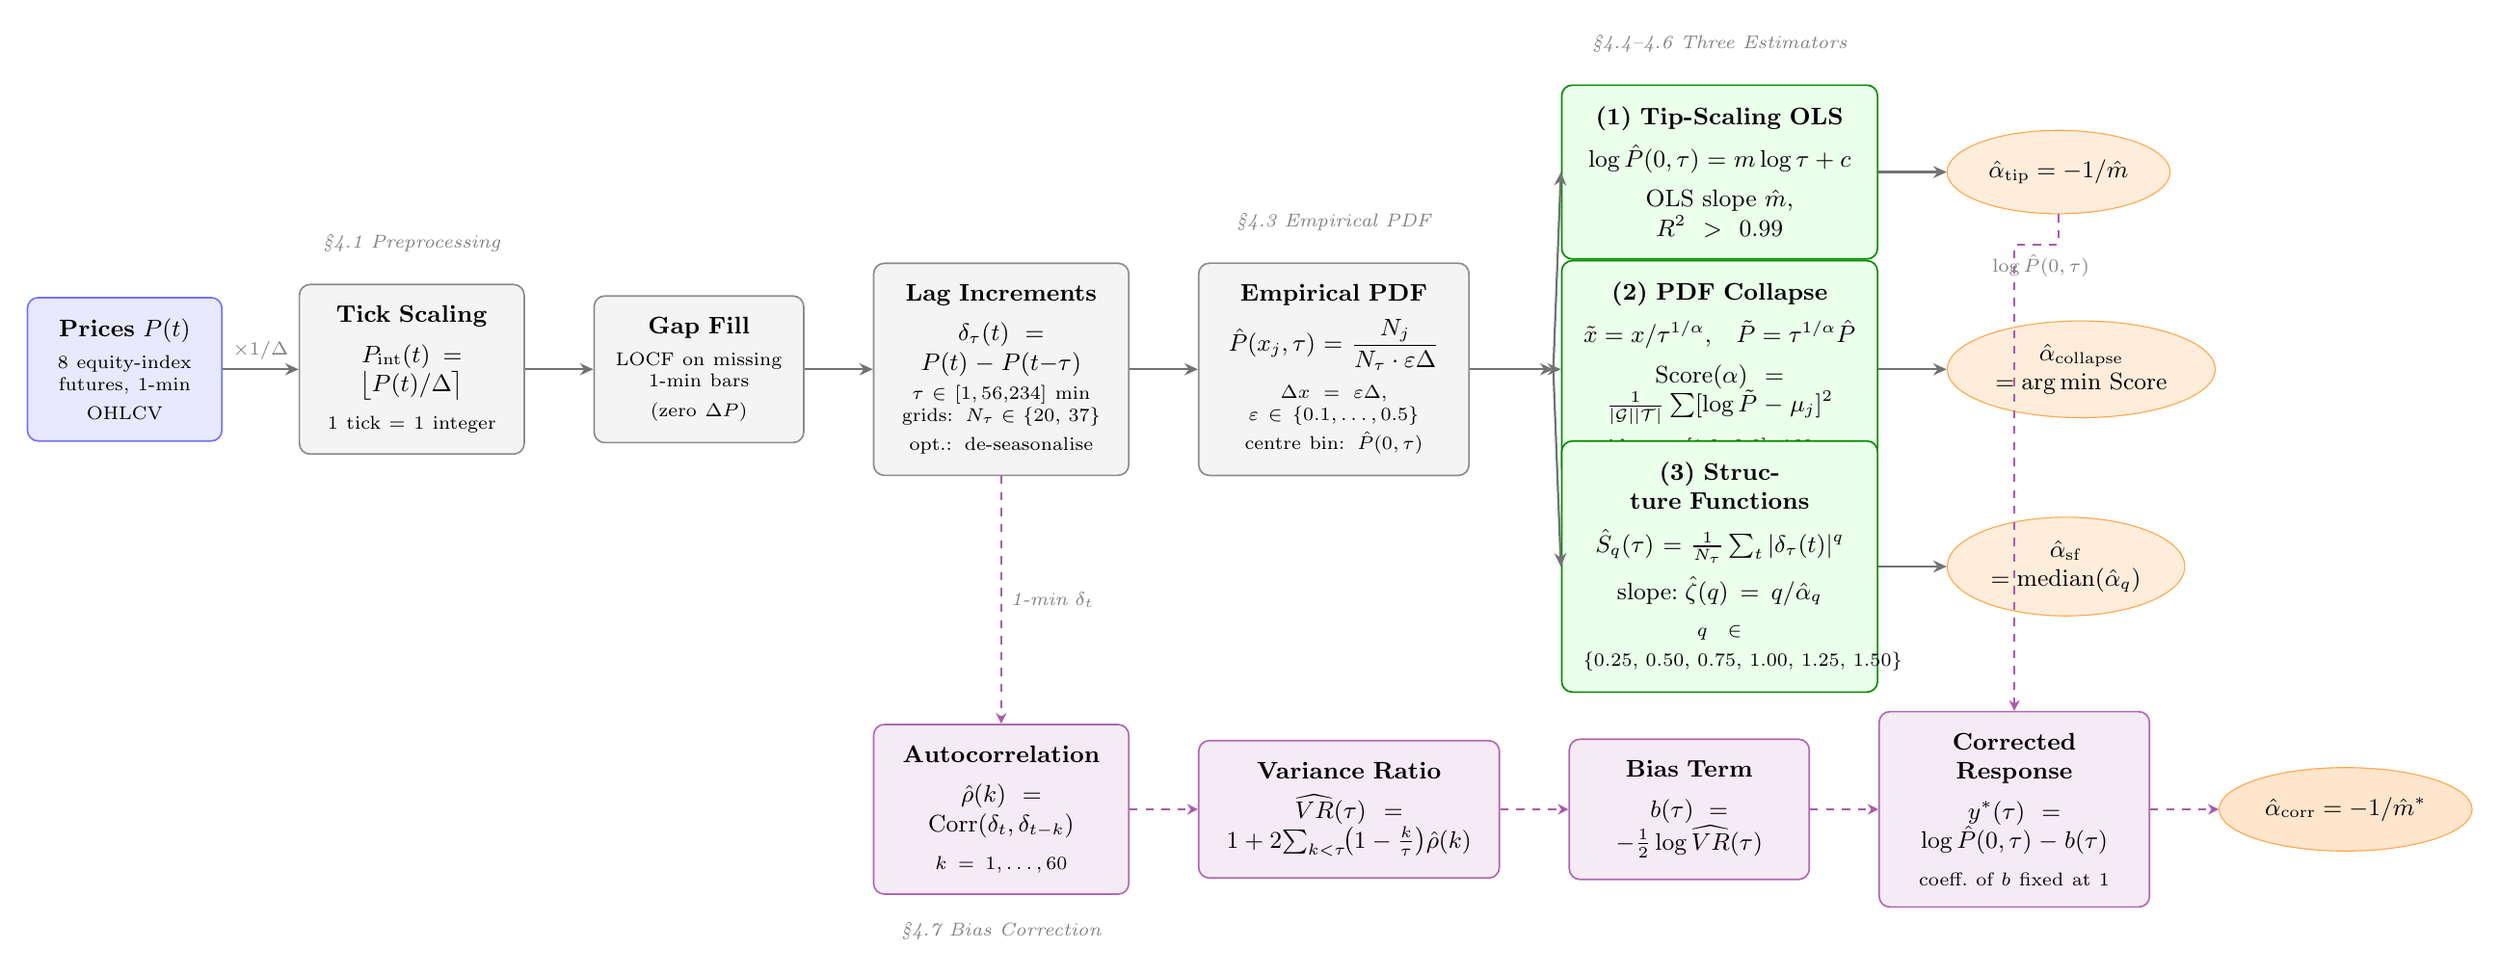
\begin{tikzpicture}[
  databox/.style  = {rectangle, rounded corners=4pt,
                     draw=blue!55, fill=blue!9, semithick,
                     align=center, font=\small, inner sep=8pt,
                     minimum height=1.2cm},
  procbox/.style  = {rectangle, rounded corners=4pt,
                     draw=black!45, fill=gray!9, semithick,
                     align=center, font=\small, inner sep=8pt,
                     minimum height=1.2cm},
  estimbox/.style = {rectangle, rounded corners=4pt,
                     draw=green!55!black, fill=green!8, semithick,
                     align=center, font=\small, inner sep=8pt,
                     minimum height=1.2cm},
  biasbox/.style  = {rectangle, rounded corners=4pt,
                     draw=violet!60, fill=violet!8, semithick,
                     align=center, font=\small, inner sep=8pt,
                     minimum height=1.2cm},
  resnode/.style  = {ellipse, draw=orange!70, fill=orange!14,
                     align=center, font=\small\bfseries,
                     minimum width=2.2cm, minimum height=1.1cm},
  arr/.style  = {-{Stealth[length=5pt,width=4.5pt]}, thick, black!55},
  arrv/.style = {-{Stealth[length=4pt,width=4pt]}, semithick, violet!65, dashed},
  lbl/.style  = {font=\scriptsize\itshape, text=black!50},
]

%%═══════════════════════════════════════════════════════════
%% TIER 1 — Preprocessing
%%═══════════════════════════════════════════════════════════

\node[databox, text width=2.0cm] (prices) at (0,0)
  {\textbf{Prices} $P(t)$\\[4pt]
   \scriptsize 8 equity-index\\futures, 1-min\\OHLCV};

\node[procbox, text width=2.4cm, right=1.0cm of prices] (scale)
  {\textbf{Tick Scaling}\\[4pt]
   $P_{\mathrm{int}}(t)=\bigl\lfloor P(t)/\Delta\bigr\rceil$\\[3pt]
   \scriptsize 1 tick $=$ 1 integer};

\draw[arr] (prices) -- (scale) node[midway,above,lbl]{$\times 1/\Delta$};

\node[procbox, text width=2.2cm, right=0.9cm of scale] (locf)
  {\textbf{Gap Fill}\\[4pt]
   \scriptsize LOCF on missing\\1-min bars\\(zero $\Delta P$)};

\draw[arr] (scale) -- (locf);

\node[procbox, text width=2.8cm, right=0.9cm of locf] (incr)
  {\textbf{Lag Increments}\\[4pt]
   $\delta_\tau(t)=P(t)-P(t{-}\tau)$\\[3pt]
   \scriptsize $\tau\in[1,56{,}234]$ min\\
   grids: $N_\tau\in\{20,\,37\}$\\
   opt.: de-seasonalise};

\draw[arr] (locf) -- (incr);

\node[procbox, text width=3.0cm, right=0.9cm of incr] (pdf)
  {\textbf{Empirical PDF}\\[4pt]
   $\hat{P}(x_j,\tau)=\dfrac{N_j}{N_\tau\cdot\varepsilon\Delta}$\\[5pt]
   \scriptsize $\Delta x=\varepsilon\Delta$,\;
   $\varepsilon\in\{0.1,\ldots,0.5\}$\\
   centre bin: $\hat{P}(0,\tau)$};

\draw[arr] (incr) -- (pdf);

\node[lbl, above=0.3cm of scale] {\S4.1 Preprocessing};
\node[lbl, above=0.3cm of pdf]   {\S4.3 Empirical PDF};

%%═══════════════════════════════════════════════════════════
%% TIER 2 — Three estimators
%%═══════════════════════════════════════════════════════════

\coordinate (fan) at ($(pdf.east)+(1.1,0)$);
\draw[arr] (pdf.east) -- (fan);

%% (1) Tip-Scaling OLS
\node[estimbox, text width=3.6cm, anchor=west]
  (tip) at ($(fan)+(0.1, 2.6)$)
  {\textbf{(1) Tip-Scaling OLS}\\[5pt]
   $\log\hat{P}(0,\tau) = m\log\tau + c$\\[4pt]
   OLS slope $\hat{m}$,\quad $R^2>0.99$};

\draw[arr] (fan) -- (tip.west);
\node[resnode, right=0.9cm of tip] (rtip)
  {$\hat\alpha_{\mathrm{tip}}=-1/\hat{m}$};
\draw[arr] (tip) -- (rtip);

%% (2) PDF Collapse
\node[estimbox, text width=3.6cm, anchor=west]
  (coll) at ($(fan)+(0.1, 0)$)
  {\textbf{(2) PDF Collapse}\\[5pt]
   $\tilde{x}=x/\tau^{1/\alpha}$,\quad
   $\tilde{P}=\tau^{1/\alpha}\hat{P}$\\[4pt]
   $\mathrm{Score}(\alpha)=
     \tfrac{1}{|\mathcal{G}||\mathcal{T}|}
     \sum[\log\tilde{P}-\mu_j]^2$\\[4pt]
   \scriptsize grid: $\alpha\in[1.2,\,2.8]$, 160 pts};

\draw[arr] (fan) -- (coll.west);
\node[resnode, right=0.9cm of coll] (rcoll)
  {$\hat\alpha_{\mathrm{collapse}}$\\$=\arg\min\,\mathrm{Score}$};
\draw[arr] (coll) -- (rcoll);

%% (3) Structure Functions
\node[estimbox, text width=3.6cm, anchor=west]
  (sf) at ($(fan)+(0.1,-2.6)$)
  {\textbf{(3) Structure Functions}\\[5pt]
   $\hat{S}_q(\tau)=\tfrac{1}{N_\tau}\sum_t|\delta_\tau(t)|^q$\\[4pt]
   slope:\;$\hat\zeta(q)=q/\hat\alpha_q$\\[3pt]
   \scriptsize $q\in\{0.25,\,0.50,\,0.75,\,1.00,\,1.25,\,1.50\}$};

\draw[arr] (fan) -- (sf.west);
\node[resnode, right=0.9cm of sf] (rsf)
  {$\hat\alpha_{\mathrm{sf}}$\\$=\mathrm{median}(\hat\alpha_q)$};
\draw[arr] (sf) -- (rsf);

\node[lbl, above=0.3cm of tip] {\S4.4--4.6 Three Estimators};

%%═══════════════════════════════════════════════════════════
%% TIER 3 — Bias correction
%%═══════════════════════════════════════════════════════════

\node[biasbox, text width=2.8cm] (rho) at ($(incr)+(0,-5.8)$)
  {\textbf{Autocorrelation}\\[4pt]
   $\hat\rho(k)=\mathrm{Corr}(\delta_t,\delta_{t-k})$\\[3pt]
   \scriptsize $k=1,\ldots,60$};

\node[biasbox, text width=3.4cm, right=0.9cm of rho] (vr)
  {\textbf{Variance Ratio}\\[4pt]
   $\widehat{VR}(\tau)=1+2\!\sum_{k<\tau}\!\bigl(1-\tfrac{k}{\tau}\bigr)\hat\rho(k)$};

\node[biasbox, text width=2.6cm, right=0.9cm of vr] (bt)
  {\textbf{Bias Term}\\[4pt]
   $b(\tau)=-\tfrac{1}{2}\log\widehat{VR}(\tau)$};

\node[biasbox, text width=3.0cm, right=0.9cm of bt] (ystar)
  {\textbf{Corrected Response}\\[4pt]
   $y^*(\tau)=\log\hat{P}(0,\tau)-b(\tau)$\\[3pt]
   \scriptsize coeff.\ of $b$ fixed at 1};

\node[resnode, fill=orange!20, right=0.9cm of ystar] (rcorr)
  {$\hat\alpha_{\mathrm{corr}}=-1/\hat{m}^*$};

\draw[arrv] (rho)   -- (vr);
\draw[arrv] (vr)    -- (bt);
\draw[arrv] (bt)    -- (ystar);
\draw[arrv] (ystar) -- (rcorr);

\draw[arrv] (incr.south) -- (rho.north)
  node[midway, right, lbl] {1-min $\delta_t$};

\draw[arrv] (rtip.south) -- ++(0,-0.4) -| (ystar.north)
  node[pos=0.2, below, lbl] {$\log\hat{P}(0,\tau)$};

\node[lbl, below=0.25cm of rho] {\S4.7 Bias Correction};

\end{tikzpicture}
\end{document}
}
%   \caption{...}
%   \label{fig:pipeline}
%   \end{figure*}
% ──────────────────────────────────────────────────────────────────────────────
\documentclass[tikz, border=12pt]{standalone}
\usepackage{amsmath,amssymb}
\usepackage{tikz}
\usetikzlibrary{shapes.geometric,arrows.meta,positioning,calc}

\begin{document}
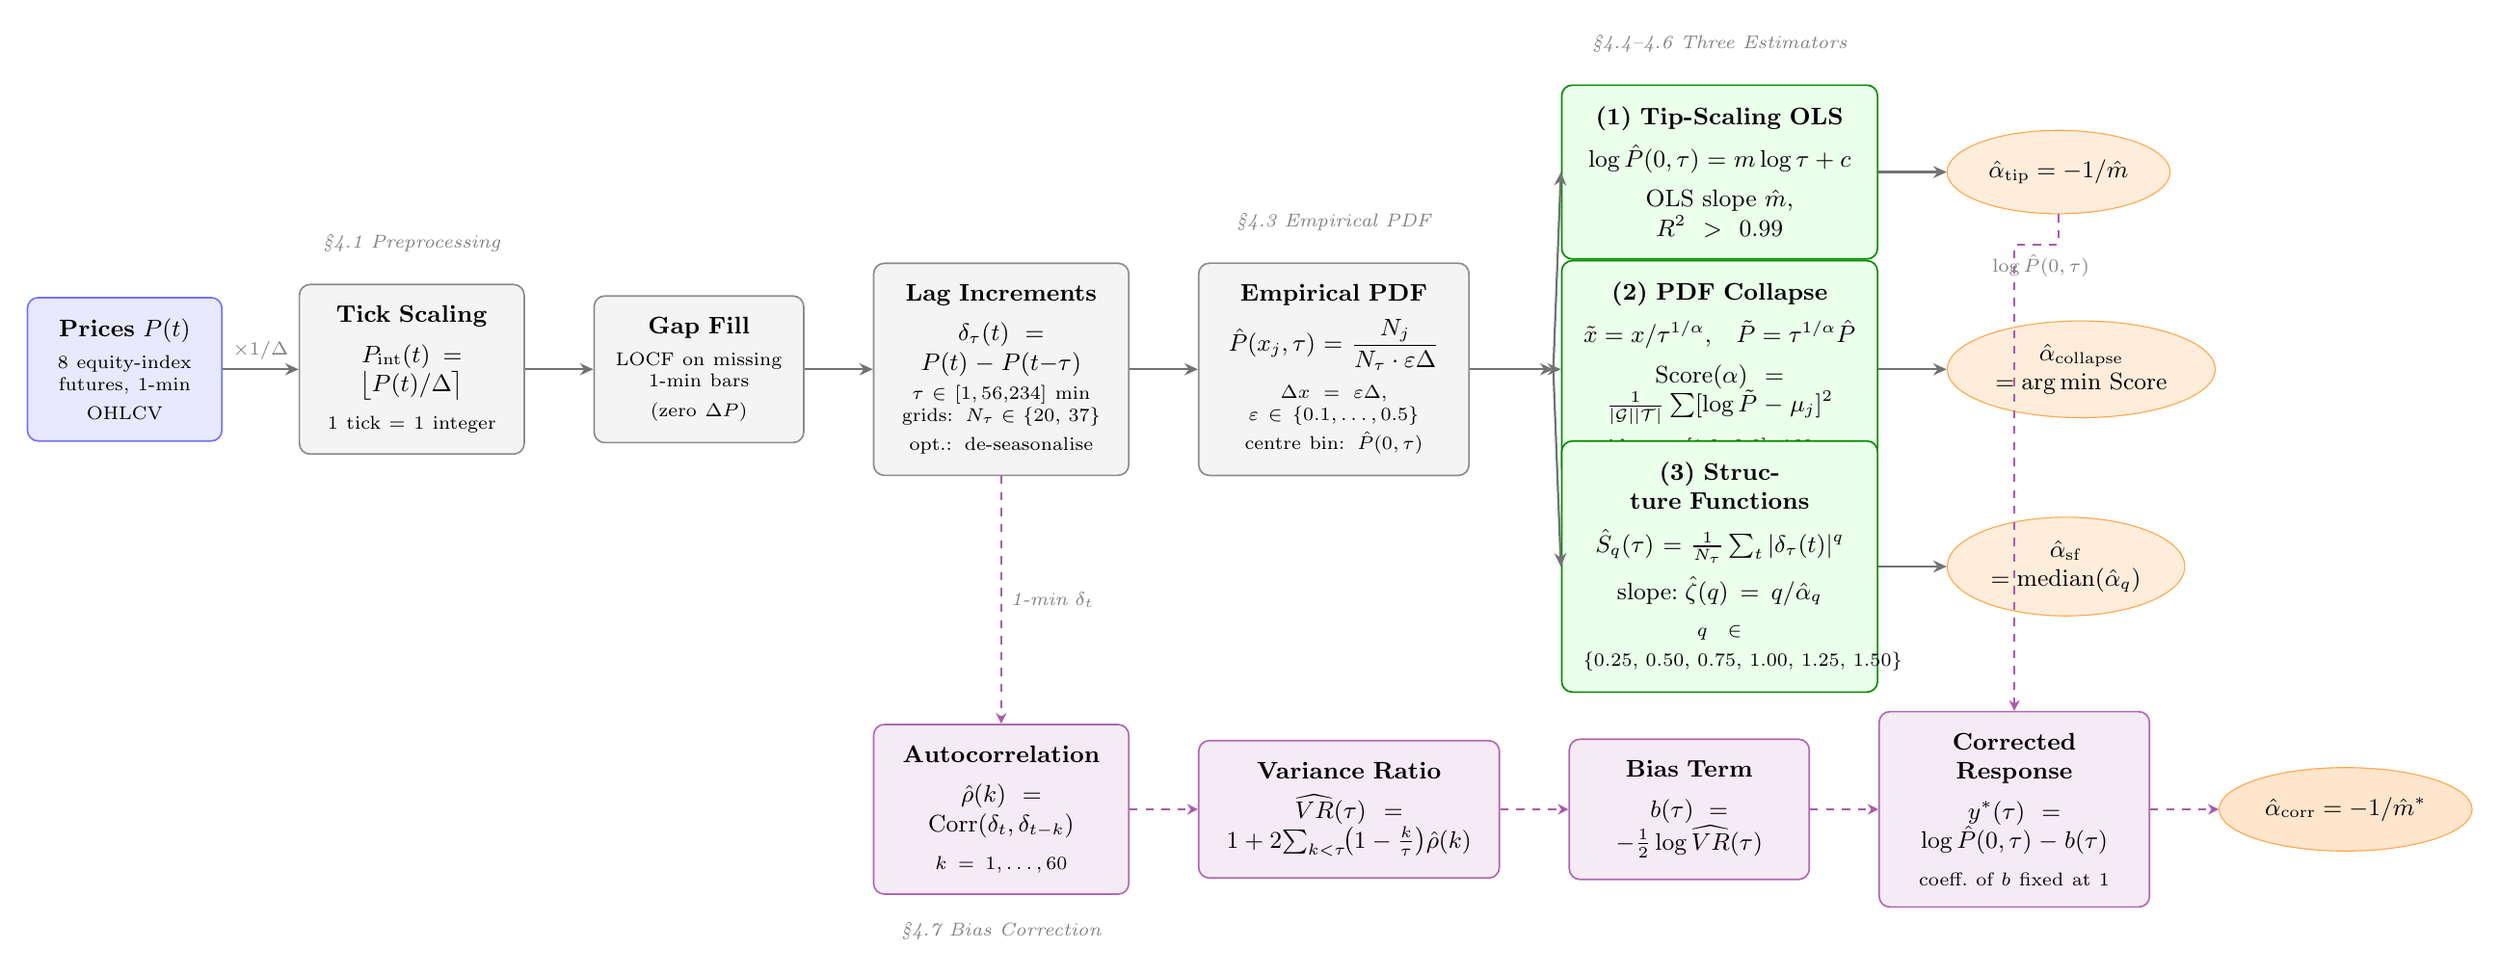
\begin{tikzpicture}[
  databox/.style  = {rectangle, rounded corners=4pt,
                     draw=blue!55, fill=blue!9, semithick,
                     align=center, font=\small, inner sep=8pt,
                     minimum height=1.2cm},
  procbox/.style  = {rectangle, rounded corners=4pt,
                     draw=black!45, fill=gray!9, semithick,
                     align=center, font=\small, inner sep=8pt,
                     minimum height=1.2cm},
  estimbox/.style = {rectangle, rounded corners=4pt,
                     draw=green!55!black, fill=green!8, semithick,
                     align=center, font=\small, inner sep=8pt,
                     minimum height=1.2cm},
  biasbox/.style  = {rectangle, rounded corners=4pt,
                     draw=violet!60, fill=violet!8, semithick,
                     align=center, font=\small, inner sep=8pt,
                     minimum height=1.2cm},
  resnode/.style  = {ellipse, draw=orange!70, fill=orange!14,
                     align=center, font=\small\bfseries,
                     minimum width=2.2cm, minimum height=1.1cm},
  arr/.style  = {-{Stealth[length=5pt,width=4.5pt]}, thick, black!55},
  arrv/.style = {-{Stealth[length=4pt,width=4pt]}, semithick, violet!65, dashed},
  lbl/.style  = {font=\scriptsize\itshape, text=black!50},
]

%%═══════════════════════════════════════════════════════════
%% TIER 1 — Preprocessing
%%═══════════════════════════════════════════════════════════

\node[databox, text width=2.0cm] (prices) at (0,0)
  {\textbf{Prices} $P(t)$\\[4pt]
   \scriptsize 8 equity-index\\futures, 1-min\\OHLCV};

\node[procbox, text width=2.4cm, right=1.0cm of prices] (scale)
  {\textbf{Tick Scaling}\\[4pt]
   $P_{\mathrm{int}}(t)=\bigl\lfloor P(t)/\Delta\bigr\rceil$\\[3pt]
   \scriptsize 1 tick $=$ 1 integer};

\draw[arr] (prices) -- (scale) node[midway,above,lbl]{$\times 1/\Delta$};

\node[procbox, text width=2.2cm, right=0.9cm of scale] (locf)
  {\textbf{Gap Fill}\\[4pt]
   \scriptsize LOCF on missing\\1-min bars\\(zero $\Delta P$)};

\draw[arr] (scale) -- (locf);

\node[procbox, text width=2.8cm, right=0.9cm of locf] (incr)
  {\textbf{Lag Increments}\\[4pt]
   $\delta_\tau(t)=P(t)-P(t{-}\tau)$\\[3pt]
   \scriptsize $\tau\in[1,56{,}234]$ min\\
   grids: $N_\tau\in\{20,\,37\}$\\
   opt.: de-seasonalise};

\draw[arr] (locf) -- (incr);

\node[procbox, text width=3.0cm, right=0.9cm of incr] (pdf)
  {\textbf{Empirical PDF}\\[4pt]
   $\hat{P}(x_j,\tau)=\dfrac{N_j}{N_\tau\cdot\varepsilon\Delta}$\\[5pt]
   \scriptsize $\Delta x=\varepsilon\Delta$,\;
   $\varepsilon\in\{0.1,\ldots,0.5\}$\\
   centre bin: $\hat{P}(0,\tau)$};

\draw[arr] (incr) -- (pdf);

\node[lbl, above=0.3cm of scale] {\S4.1 Preprocessing};
\node[lbl, above=0.3cm of pdf]   {\S4.3 Empirical PDF};

%%═══════════════════════════════════════════════════════════
%% TIER 2 — Three estimators
%%═══════════════════════════════════════════════════════════

\coordinate (fan) at ($(pdf.east)+(1.1,0)$);
\draw[arr] (pdf.east) -- (fan);

%% (1) Tip-Scaling OLS
\node[estimbox, text width=3.6cm, anchor=west]
  (tip) at ($(fan)+(0.1, 2.6)$)
  {\textbf{(1) Tip-Scaling OLS}\\[5pt]
   $\log\hat{P}(0,\tau) = m\log\tau + c$\\[4pt]
   OLS slope $\hat{m}$,\quad $R^2>0.99$};

\draw[arr] (fan) -- (tip.west);
\node[resnode, right=0.9cm of tip] (rtip)
  {$\hat\alpha_{\mathrm{tip}}=-1/\hat{m}$};
\draw[arr] (tip) -- (rtip);

%% (2) PDF Collapse
\node[estimbox, text width=3.6cm, anchor=west]
  (coll) at ($(fan)+(0.1, 0)$)
  {\textbf{(2) PDF Collapse}\\[5pt]
   $\tilde{x}=x/\tau^{1/\alpha}$,\quad
   $\tilde{P}=\tau^{1/\alpha}\hat{P}$\\[4pt]
   $\mathrm{Score}(\alpha)=
     \tfrac{1}{|\mathcal{G}||\mathcal{T}|}
     \sum[\log\tilde{P}-\mu_j]^2$\\[4pt]
   \scriptsize grid: $\alpha\in[1.2,\,2.8]$, 160 pts};

\draw[arr] (fan) -- (coll.west);
\node[resnode, right=0.9cm of coll] (rcoll)
  {$\hat\alpha_{\mathrm{collapse}}$\\$=\arg\min\,\mathrm{Score}$};
\draw[arr] (coll) -- (rcoll);

%% (3) Structure Functions
\node[estimbox, text width=3.6cm, anchor=west]
  (sf) at ($(fan)+(0.1,-2.6)$)
  {\textbf{(3) Structure Functions}\\[5pt]
   $\hat{S}_q(\tau)=\tfrac{1}{N_\tau}\sum_t|\delta_\tau(t)|^q$\\[4pt]
   slope:\;$\hat\zeta(q)=q/\hat\alpha_q$\\[3pt]
   \scriptsize $q\in\{0.25,\,0.50,\,0.75,\,1.00,\,1.25,\,1.50\}$};

\draw[arr] (fan) -- (sf.west);
\node[resnode, right=0.9cm of sf] (rsf)
  {$\hat\alpha_{\mathrm{sf}}$\\$=\mathrm{median}(\hat\alpha_q)$};
\draw[arr] (sf) -- (rsf);

\node[lbl, above=0.3cm of tip] {\S4.4--4.6 Three Estimators};

%%═══════════════════════════════════════════════════════════
%% TIER 3 — Bias correction
%%═══════════════════════════════════════════════════════════

\node[biasbox, text width=2.8cm] (rho) at ($(incr)+(0,-5.8)$)
  {\textbf{Autocorrelation}\\[4pt]
   $\hat\rho(k)=\mathrm{Corr}(\delta_t,\delta_{t-k})$\\[3pt]
   \scriptsize $k=1,\ldots,60$};

\node[biasbox, text width=3.4cm, right=0.9cm of rho] (vr)
  {\textbf{Variance Ratio}\\[4pt]
   $\widehat{VR}(\tau)=1+2\!\sum_{k<\tau}\!\bigl(1-\tfrac{k}{\tau}\bigr)\hat\rho(k)$};

\node[biasbox, text width=2.6cm, right=0.9cm of vr] (bt)
  {\textbf{Bias Term}\\[4pt]
   $b(\tau)=-\tfrac{1}{2}\log\widehat{VR}(\tau)$};

\node[biasbox, text width=3.0cm, right=0.9cm of bt] (ystar)
  {\textbf{Corrected Response}\\[4pt]
   $y^*(\tau)=\log\hat{P}(0,\tau)-b(\tau)$\\[3pt]
   \scriptsize coeff.\ of $b$ fixed at 1};

\node[resnode, fill=orange!20, right=0.9cm of ystar] (rcorr)
  {$\hat\alpha_{\mathrm{corr}}=-1/\hat{m}^*$};

\draw[arrv] (rho)   -- (vr);
\draw[arrv] (vr)    -- (bt);
\draw[arrv] (bt)    -- (ystar);
\draw[arrv] (ystar) -- (rcorr);

\draw[arrv] (incr.south) -- (rho.north)
  node[midway, right, lbl] {1-min $\delta_t$};

\draw[arrv] (rtip.south) -- ++(0,-0.4) -| (ystar.north)
  node[pos=0.2, below, lbl] {$\log\hat{P}(0,\tau)$};

\node[lbl, below=0.25cm of rho] {\S4.7 Bias Correction};

\end{tikzpicture}
\end{document}
}
%   \caption{...}
%   \label{fig:pipeline}
%   \end{figure*}
% ──────────────────────────────────────────────────────────────────────────────
\documentclass[tikz, border=12pt]{standalone}
\usepackage{amsmath,amssymb}
\usepackage{tikz}
\usetikzlibrary{shapes.geometric,arrows.meta,positioning,calc}

\begin{document}
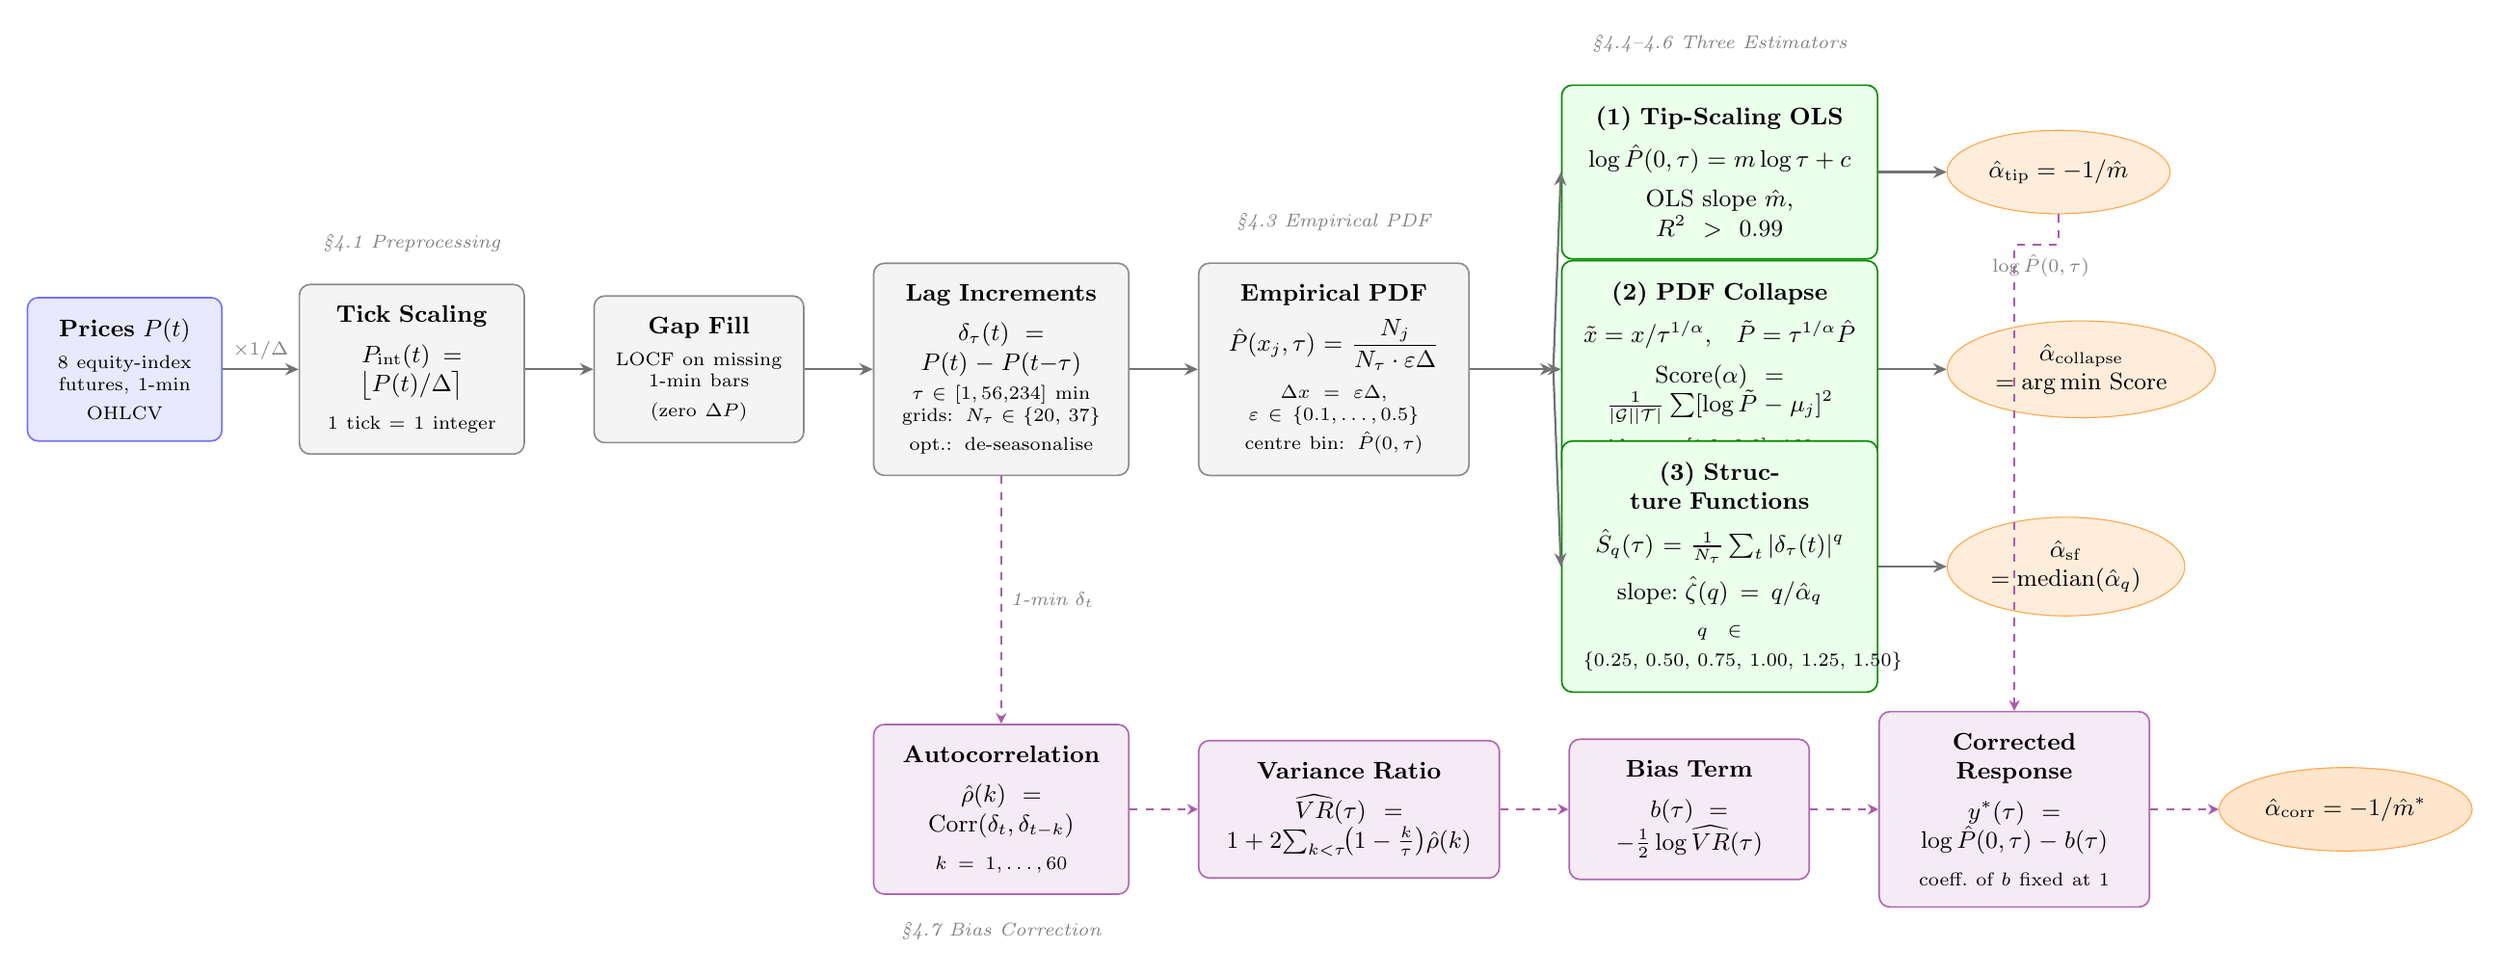
\begin{tikzpicture}[
  databox/.style  = {rectangle, rounded corners=4pt,
                     draw=blue!55, fill=blue!9, semithick,
                     align=center, font=\small, inner sep=8pt,
                     minimum height=1.2cm},
  procbox/.style  = {rectangle, rounded corners=4pt,
                     draw=black!45, fill=gray!9, semithick,
                     align=center, font=\small, inner sep=8pt,
                     minimum height=1.2cm},
  estimbox/.style = {rectangle, rounded corners=4pt,
                     draw=green!55!black, fill=green!8, semithick,
                     align=center, font=\small, inner sep=8pt,
                     minimum height=1.2cm},
  biasbox/.style  = {rectangle, rounded corners=4pt,
                     draw=violet!60, fill=violet!8, semithick,
                     align=center, font=\small, inner sep=8pt,
                     minimum height=1.2cm},
  resnode/.style  = {ellipse, draw=orange!70, fill=orange!14,
                     align=center, font=\small\bfseries,
                     minimum width=2.2cm, minimum height=1.1cm},
  arr/.style  = {-{Stealth[length=5pt,width=4.5pt]}, thick, black!55},
  arrv/.style = {-{Stealth[length=4pt,width=4pt]}, semithick, violet!65, dashed},
  lbl/.style  = {font=\scriptsize\itshape, text=black!50},
]

%%═══════════════════════════════════════════════════════════
%% TIER 1 — Preprocessing
%%═══════════════════════════════════════════════════════════

\node[databox, text width=2.0cm] (prices) at (0,0)
  {\textbf{Prices} $P(t)$\\[4pt]
   \scriptsize 8 equity-index\\futures, 1-min\\OHLCV};

\node[procbox, text width=2.4cm, right=1.0cm of prices] (scale)
  {\textbf{Tick Scaling}\\[4pt]
   $P_{\mathrm{int}}(t)=\bigl\lfloor P(t)/\Delta\bigr\rceil$\\[3pt]
   \scriptsize 1 tick $=$ 1 integer};

\draw[arr] (prices) -- (scale) node[midway,above,lbl]{$\times 1/\Delta$};

\node[procbox, text width=2.2cm, right=0.9cm of scale] (locf)
  {\textbf{Gap Fill}\\[4pt]
   \scriptsize LOCF on missing\\1-min bars\\(zero $\Delta P$)};

\draw[arr] (scale) -- (locf);

\node[procbox, text width=2.8cm, right=0.9cm of locf] (incr)
  {\textbf{Lag Increments}\\[4pt]
   $\delta_\tau(t)=P(t)-P(t{-}\tau)$\\[3pt]
   \scriptsize $\tau\in[1,56{,}234]$ min\\
   grids: $N_\tau\in\{20,\,37\}$\\
   opt.: de-seasonalise};

\draw[arr] (locf) -- (incr);

\node[procbox, text width=3.0cm, right=0.9cm of incr] (pdf)
  {\textbf{Empirical PDF}\\[4pt]
   $\hat{P}(x_j,\tau)=\dfrac{N_j}{N_\tau\cdot\varepsilon\Delta}$\\[5pt]
   \scriptsize $\Delta x=\varepsilon\Delta$,\;
   $\varepsilon\in\{0.1,\ldots,0.5\}$\\
   centre bin: $\hat{P}(0,\tau)$};

\draw[arr] (incr) -- (pdf);

\node[lbl, above=0.3cm of scale] {\S4.1 Preprocessing};
\node[lbl, above=0.3cm of pdf]   {\S4.3 Empirical PDF};

%%═══════════════════════════════════════════════════════════
%% TIER 2 — Three estimators
%%═══════════════════════════════════════════════════════════

\coordinate (fan) at ($(pdf.east)+(1.1,0)$);
\draw[arr] (pdf.east) -- (fan);

%% (1) Tip-Scaling OLS
\node[estimbox, text width=3.6cm, anchor=west]
  (tip) at ($(fan)+(0.1, 2.6)$)
  {\textbf{(1) Tip-Scaling OLS}\\[5pt]
   $\log\hat{P}(0,\tau) = m\log\tau + c$\\[4pt]
   OLS slope $\hat{m}$,\quad $R^2>0.99$};

\draw[arr] (fan) -- (tip.west);
\node[resnode, right=0.9cm of tip] (rtip)
  {$\hat\alpha_{\mathrm{tip}}=-1/\hat{m}$};
\draw[arr] (tip) -- (rtip);

%% (2) PDF Collapse
\node[estimbox, text width=3.6cm, anchor=west]
  (coll) at ($(fan)+(0.1, 0)$)
  {\textbf{(2) PDF Collapse}\\[5pt]
   $\tilde{x}=x/\tau^{1/\alpha}$,\quad
   $\tilde{P}=\tau^{1/\alpha}\hat{P}$\\[4pt]
   $\mathrm{Score}(\alpha)=
     \tfrac{1}{|\mathcal{G}||\mathcal{T}|}
     \sum[\log\tilde{P}-\mu_j]^2$\\[4pt]
   \scriptsize grid: $\alpha\in[1.2,\,2.8]$, 160 pts};

\draw[arr] (fan) -- (coll.west);
\node[resnode, right=0.9cm of coll] (rcoll)
  {$\hat\alpha_{\mathrm{collapse}}$\\$=\arg\min\,\mathrm{Score}$};
\draw[arr] (coll) -- (rcoll);

%% (3) Structure Functions
\node[estimbox, text width=3.6cm, anchor=west]
  (sf) at ($(fan)+(0.1,-2.6)$)
  {\textbf{(3) Structure Functions}\\[5pt]
   $\hat{S}_q(\tau)=\tfrac{1}{N_\tau}\sum_t|\delta_\tau(t)|^q$\\[4pt]
   slope:\;$\hat\zeta(q)=q/\hat\alpha_q$\\[3pt]
   \scriptsize $q\in\{0.25,\,0.50,\,0.75,\,1.00,\,1.25,\,1.50\}$};

\draw[arr] (fan) -- (sf.west);
\node[resnode, right=0.9cm of sf] (rsf)
  {$\hat\alpha_{\mathrm{sf}}$\\$=\mathrm{median}(\hat\alpha_q)$};
\draw[arr] (sf) -- (rsf);

\node[lbl, above=0.3cm of tip] {\S4.4--4.6 Three Estimators};

%%═══════════════════════════════════════════════════════════
%% TIER 3 — Bias correction
%%═══════════════════════════════════════════════════════════

\node[biasbox, text width=2.8cm] (rho) at ($(incr)+(0,-5.8)$)
  {\textbf{Autocorrelation}\\[4pt]
   $\hat\rho(k)=\mathrm{Corr}(\delta_t,\delta_{t-k})$\\[3pt]
   \scriptsize $k=1,\ldots,60$};

\node[biasbox, text width=3.4cm, right=0.9cm of rho] (vr)
  {\textbf{Variance Ratio}\\[4pt]
   $\widehat{VR}(\tau)=1+2\!\sum_{k<\tau}\!\bigl(1-\tfrac{k}{\tau}\bigr)\hat\rho(k)$};

\node[biasbox, text width=2.6cm, right=0.9cm of vr] (bt)
  {\textbf{Bias Term}\\[4pt]
   $b(\tau)=-\tfrac{1}{2}\log\widehat{VR}(\tau)$};

\node[biasbox, text width=3.0cm, right=0.9cm of bt] (ystar)
  {\textbf{Corrected Response}\\[4pt]
   $y^*(\tau)=\log\hat{P}(0,\tau)-b(\tau)$\\[3pt]
   \scriptsize coeff.\ of $b$ fixed at 1};

\node[resnode, fill=orange!20, right=0.9cm of ystar] (rcorr)
  {$\hat\alpha_{\mathrm{corr}}=-1/\hat{m}^*$};

\draw[arrv] (rho)   -- (vr);
\draw[arrv] (vr)    -- (bt);
\draw[arrv] (bt)    -- (ystar);
\draw[arrv] (ystar) -- (rcorr);

\draw[arrv] (incr.south) -- (rho.north)
  node[midway, right, lbl] {1-min $\delta_t$};

\draw[arrv] (rtip.south) -- ++(0,-0.4) -| (ystar.north)
  node[pos=0.2, below, lbl] {$\log\hat{P}(0,\tau)$};

\node[lbl, below=0.25cm of rho] {\S4.7 Bias Correction};

\end{tikzpicture}
\end{document}
}
%   \caption{...}
%   \label{fig:pipeline}
%   \end{figure*}
% ──────────────────────────────────────────────────────────────────────────────
\documentclass[tikz, border=12pt]{standalone}
\usepackage{amsmath,amssymb}
\usepackage{tikz}
\usetikzlibrary{shapes.geometric,arrows.meta,positioning,calc}

\begin{document}
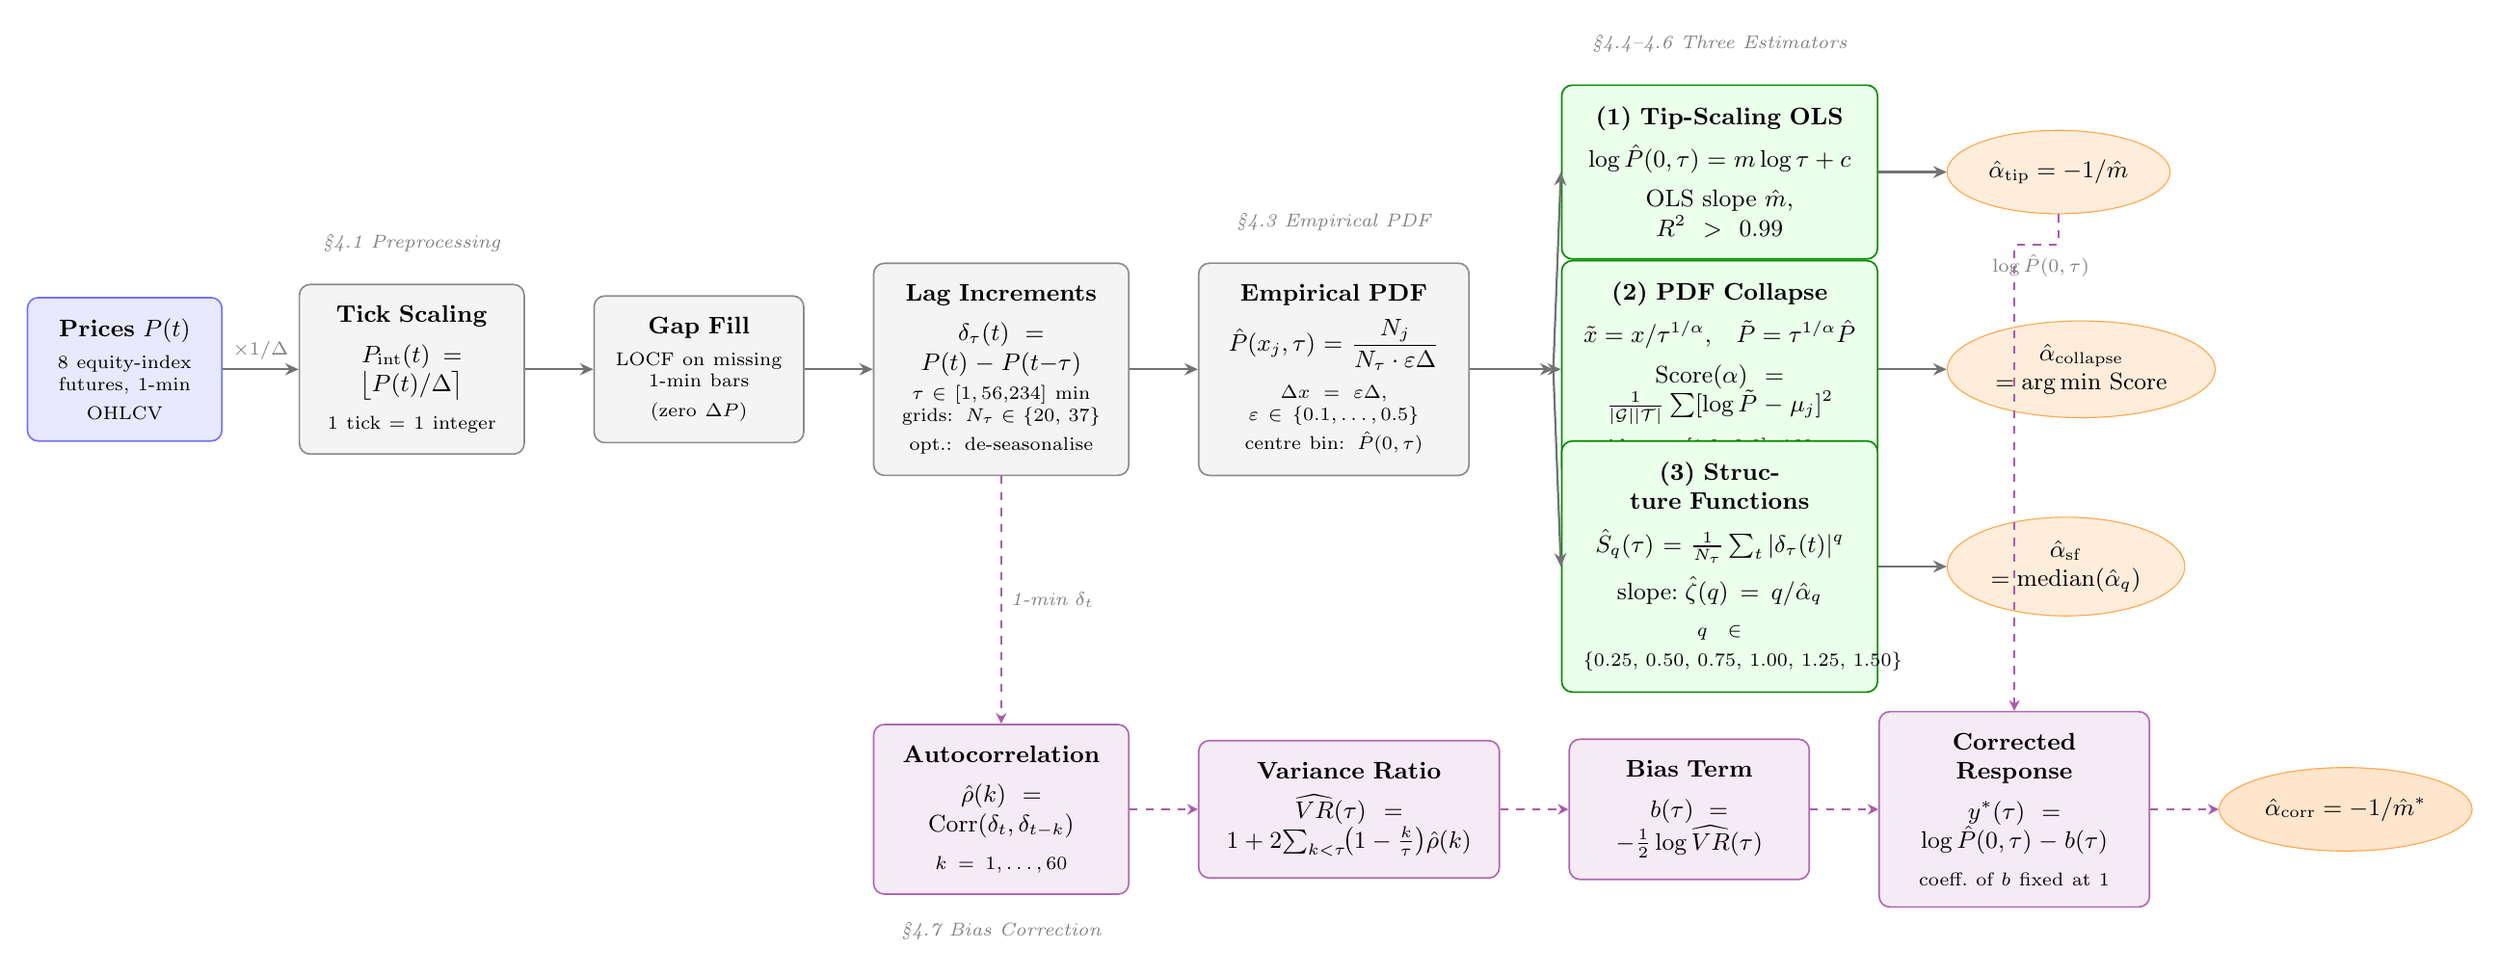
\begin{tikzpicture}[
  databox/.style  = {rectangle, rounded corners=4pt,
                     draw=blue!55, fill=blue!9, semithick,
                     align=center, font=\small, inner sep=8pt,
                     minimum height=1.2cm},
  procbox/.style  = {rectangle, rounded corners=4pt,
                     draw=black!45, fill=gray!9, semithick,
                     align=center, font=\small, inner sep=8pt,
                     minimum height=1.2cm},
  estimbox/.style = {rectangle, rounded corners=4pt,
                     draw=green!55!black, fill=green!8, semithick,
                     align=center, font=\small, inner sep=8pt,
                     minimum height=1.2cm},
  biasbox/.style  = {rectangle, rounded corners=4pt,
                     draw=violet!60, fill=violet!8, semithick,
                     align=center, font=\small, inner sep=8pt,
                     minimum height=1.2cm},
  resnode/.style  = {ellipse, draw=orange!70, fill=orange!14,
                     align=center, font=\small\bfseries,
                     minimum width=2.2cm, minimum height=1.1cm},
  arr/.style  = {-{Stealth[length=5pt,width=4.5pt]}, thick, black!55},
  arrv/.style = {-{Stealth[length=4pt,width=4pt]}, semithick, violet!65, dashed},
  lbl/.style  = {font=\scriptsize\itshape, text=black!50},
]

%%═══════════════════════════════════════════════════════════
%% TIER 1 — Preprocessing
%%═══════════════════════════════════════════════════════════

\node[databox, text width=2.0cm] (prices) at (0,0)
  {\textbf{Prices} $P(t)$\\[4pt]
   \scriptsize 8 equity-index\\futures, 1-min\\OHLCV};

\node[procbox, text width=2.4cm, right=1.0cm of prices] (scale)
  {\textbf{Tick Scaling}\\[4pt]
   $P_{\mathrm{int}}(t)=\bigl\lfloor P(t)/\Delta\bigr\rceil$\\[3pt]
   \scriptsize 1 tick $=$ 1 integer};

\draw[arr] (prices) -- (scale) node[midway,above,lbl]{$\times 1/\Delta$};

\node[procbox, text width=2.2cm, right=0.9cm of scale] (locf)
  {\textbf{Gap Fill}\\[4pt]
   \scriptsize LOCF on missing\\1-min bars\\(zero $\Delta P$)};

\draw[arr] (scale) -- (locf);

\node[procbox, text width=2.8cm, right=0.9cm of locf] (incr)
  {\textbf{Lag Increments}\\[4pt]
   $\delta_\tau(t)=P(t)-P(t{-}\tau)$\\[3pt]
   \scriptsize $\tau\in[1,56{,}234]$ min\\
   grids: $N_\tau\in\{20,\,37\}$\\
   opt.: de-seasonalise};

\draw[arr] (locf) -- (incr);

\node[procbox, text width=3.0cm, right=0.9cm of incr] (pdf)
  {\textbf{Empirical PDF}\\[4pt]
   $\hat{P}(x_j,\tau)=\dfrac{N_j}{N_\tau\cdot\varepsilon\Delta}$\\[5pt]
   \scriptsize $\Delta x=\varepsilon\Delta$,\;
   $\varepsilon\in\{0.1,\ldots,0.5\}$\\
   centre bin: $\hat{P}(0,\tau)$};

\draw[arr] (incr) -- (pdf);

\node[lbl, above=0.3cm of scale] {\S4.1 Preprocessing};
\node[lbl, above=0.3cm of pdf]   {\S4.3 Empirical PDF};

%%═══════════════════════════════════════════════════════════
%% TIER 2 — Three estimators
%%═══════════════════════════════════════════════════════════

\coordinate (fan) at ($(pdf.east)+(1.1,0)$);
\draw[arr] (pdf.east) -- (fan);

%% (1) Tip-Scaling OLS
\node[estimbox, text width=3.6cm, anchor=west]
  (tip) at ($(fan)+(0.1, 2.6)$)
  {\textbf{(1) Tip-Scaling OLS}\\[5pt]
   $\log\hat{P}(0,\tau) = m\log\tau + c$\\[4pt]
   OLS slope $\hat{m}$,\quad $R^2>0.99$};

\draw[arr] (fan) -- (tip.west);
\node[resnode, right=0.9cm of tip] (rtip)
  {$\hat\alpha_{\mathrm{tip}}=-1/\hat{m}$};
\draw[arr] (tip) -- (rtip);

%% (2) PDF Collapse
\node[estimbox, text width=3.6cm, anchor=west]
  (coll) at ($(fan)+(0.1, 0)$)
  {\textbf{(2) PDF Collapse}\\[5pt]
   $\tilde{x}=x/\tau^{1/\alpha}$,\quad
   $\tilde{P}=\tau^{1/\alpha}\hat{P}$\\[4pt]
   $\mathrm{Score}(\alpha)=
     \tfrac{1}{|\mathcal{G}||\mathcal{T}|}
     \sum[\log\tilde{P}-\mu_j]^2$\\[4pt]
   \scriptsize grid: $\alpha\in[1.2,\,2.8]$, 160 pts};

\draw[arr] (fan) -- (coll.west);
\node[resnode, right=0.9cm of coll] (rcoll)
  {$\hat\alpha_{\mathrm{collapse}}$\\$=\arg\min\,\mathrm{Score}$};
\draw[arr] (coll) -- (rcoll);

%% (3) Structure Functions
\node[estimbox, text width=3.6cm, anchor=west]
  (sf) at ($(fan)+(0.1,-2.6)$)
  {\textbf{(3) Structure Functions}\\[5pt]
   $\hat{S}_q(\tau)=\tfrac{1}{N_\tau}\sum_t|\delta_\tau(t)|^q$\\[4pt]
   slope:\;$\hat\zeta(q)=q/\hat\alpha_q$\\[3pt]
   \scriptsize $q\in\{0.25,\,0.50,\,0.75,\,1.00,\,1.25,\,1.50\}$};

\draw[arr] (fan) -- (sf.west);
\node[resnode, right=0.9cm of sf] (rsf)
  {$\hat\alpha_{\mathrm{sf}}$\\$=\mathrm{median}(\hat\alpha_q)$};
\draw[arr] (sf) -- (rsf);

\node[lbl, above=0.3cm of tip] {\S4.4--4.6 Three Estimators};

%%═══════════════════════════════════════════════════════════
%% TIER 3 — Bias correction
%%═══════════════════════════════════════════════════════════

\node[biasbox, text width=2.8cm] (rho) at ($(incr)+(0,-5.8)$)
  {\textbf{Autocorrelation}\\[4pt]
   $\hat\rho(k)=\mathrm{Corr}(\delta_t,\delta_{t-k})$\\[3pt]
   \scriptsize $k=1,\ldots,60$};

\node[biasbox, text width=3.4cm, right=0.9cm of rho] (vr)
  {\textbf{Variance Ratio}\\[4pt]
   $\widehat{VR}(\tau)=1+2\!\sum_{k<\tau}\!\bigl(1-\tfrac{k}{\tau}\bigr)\hat\rho(k)$};

\node[biasbox, text width=2.6cm, right=0.9cm of vr] (bt)
  {\textbf{Bias Term}\\[4pt]
   $b(\tau)=-\tfrac{1}{2}\log\widehat{VR}(\tau)$};

\node[biasbox, text width=3.0cm, right=0.9cm of bt] (ystar)
  {\textbf{Corrected Response}\\[4pt]
   $y^*(\tau)=\log\hat{P}(0,\tau)-b(\tau)$\\[3pt]
   \scriptsize coeff.\ of $b$ fixed at 1};

\node[resnode, fill=orange!20, right=0.9cm of ystar] (rcorr)
  {$\hat\alpha_{\mathrm{corr}}=-1/\hat{m}^*$};

\draw[arrv] (rho)   -- (vr);
\draw[arrv] (vr)    -- (bt);
\draw[arrv] (bt)    -- (ystar);
\draw[arrv] (ystar) -- (rcorr);

\draw[arrv] (incr.south) -- (rho.north)
  node[midway, right, lbl] {1-min $\delta_t$};

\draw[arrv] (rtip.south) -- ++(0,-0.4) -| (ystar.north)
  node[pos=0.2, below, lbl] {$\log\hat{P}(0,\tau)$};

\node[lbl, below=0.25cm of rho] {\S4.7 Bias Correction};

\end{tikzpicture}
\end{document}
